\chapter{Data commonly used in species distribution models}
\label{ch:DataCommonlyUsedInSpeciesDistributionModels}
\section{Predictor data}
To process the spatial data in this raster we will use \texttt{R} as a geographic information system (GIS). To do this we rely on the \textsc{raster} \parencite{raster} and \textsc{sp} \parencite{sp} packages. Although this chapter is only a small piece of the thesis the data-preparation is the most labour intensive part of it. 


\begin{figure}[!htb]
\centering
\includegraphics[scale=0.5]{VectorGraphics/DataScheme.png}
\caption{\label{fig:DataCommonlyUsedInSpeciesDistributionModels:DataScheme}Visualization of the preprocessing of the raster data.}
\end{figure}

\subsection{Vegetation continuous fields}
The Vegetation Continuous Fields (VCF) data-set contains values between $0$ and $100$. 
250m grid. These values 
\subsection{Bioclimatic variables}
Bioclimatic variables are a set of variables that describe ecologically relevant climate patterns. \todo[inline]{find a citation} The definitions of each of the $19$ bioclimatic variables can be found in Table \ref{table:Bioclim}. The bioclimatic variables can be derived from monthly minimum, maximum, and average temperature and precipitation data.

\begin{table}[htb]
\begin{tabular}{ll}
\toprule
Variable name & Explanation \\ 
\midrule
BIO1 & Annual Mean Temperature \\
BIO2 & Mean Diurnal Range (Mean of monthly $\left( \text{Temp}_{max} - \text{Temp}_{min} \right)$ \\
BIO3 & Isothermality $\left( 100 \times \frac{\text{BIO2}}{\text{BIO7}} \right)$  \\
BIO4 & Temperature Seasonality $\left(SD(\text{Temp}_{avg}) * 100\right)$ \\
BIO5 & Max Temperature of Warmest Month \\
BIO6 & Min Temperature of Coldest Month \\
BIO7 & Temperature Annual Range $\left(\text{BIO5} - \text{BIO6}\right)$ \\
BIO8 & Mean Temperature of Wettest Quarter \\
BIO9 & Mean Temperature of Driest Quarter \\
BIO10 & Mean Temperature of Warmest Quarter \\
BIO11 & Mean Temperature of Coldest Quarter \\
BIO12 & Annual Precipitation \\
BIO13 & Precipitation of Wettest Month \\
BIO14 & Precipitation of Driest Month \\
BIO15 & Precipitation Seasonality $\left( \right)$ \\
BIO16 & Precipitation of Wettest Quarter \\
BIO17 & Precipitation of Driest Quarter \\
BIO18 & Precipitation of Warmest Quarter \\
BIO19 & Precipitation of Coldest Quarter \\
\bottomrule
\end{tabular}
\caption{\label{table:Bioclim}Explanation of the bioclimatic variables.}
\end{table}

It is clear that the vectors corresponding  to BIO05, BIO6, and BIO7 are linear dependent. This linear dependence can be problematic when using classification methods and will be discussed in Chapter \ref{ch:ClassificationTechniques}.\\ 

We obtained the monthly temperature and precipitation data from the PRISM database \parencite{PRISM}. The PRISM database has a grid cell size of 0.00833 degrees and the datum of the layers is WGS84. To calculate the bioclimatic variables we adapted the \textsc{biovars} function from the \textsc{dismo} package \parencite{dismo}. The \textsc{biovars} function from the \textsc{dismo} package does not allow the user to provide a layer of the mean temperature, instead it uses the average of the minimum and maximum temperature in each cell in the calculations requiring the mean temperature. Our adaptation does use the mean temperature layers and should be slightly more realistic.

\subsection{NDVI}

\subsection{Digital elevation model}

\subsection{Land cover}
\todo[inline]{note that the sum of the variables = 1 => design matrix will not have full rank ...}

\section{Outcome data}
\subsection{Species considered}

\begin{sidewaystable}[!htb]
\centering
\begin{tabular}{l l c c c c c }
\toprule
Species & common name & US & West Coast & East Coast & Western US & Southeastern US \\
\midrule
Aesculus glabra & Ohio buckeye  &  \ding{51} \\
Juniperus osteosperma & Utah juniper  & & &  \ding{51}\\
Quercus ilicifolia & bear oak  & & &  \ding{51}  \\
Salix caroliniana & coastal plain willow  &  \ding{51}  \\
Sequoia sempervirens& coast redwood & &  \ding{51}  \\
\\
Agkistrodon contortrix Linnaeus & copperhead snake   &  \ding{51}  \\
Geomys pinetis Rafinesque & southeastern pocket gopher  &&&& &  \ding{51}  \\
Pituophis catenifer catenifer & Pacific gopher snake  &  &  \ding{51}  \\
Sorex pacificus & Pacific shrew &  &  \ding{51}  \\
Sylvilagus nuttallii & mountain cottontail  & & &  &  \ding{51}  \\
\bottomrule
\end{tabular}
\caption{\label{table:Species}The different species studied and the study extent.}
\end{sidewaystable}

\begin{figure}[!htb]
\centering
\includegraphics[scale=0.6]{Plots/StudyExtent.png}
\end{figure}


\subsection{Global Biodiversity Information Facility}



\section{Spatial scale}
\label{sec:SpatialScale}

\todo[inline]{cite Fine-scale environmental variation in species distribution modelling ...}